\begin{frame}{Bi-Hyperimmune sets}
  \begin{define}
    $X\subseteq\omega$ is \textbf{hyperimmune} if there is no computable
    function $f$ such that $f(n)>p_X(n)$ for every $n\in\omega$.
  \end{define}

  \begin{define}
    $X$ is \textbf{bi-hyperimmune} if both $X$ and $\bar{X}$ are hyperimmune.
  \end{define}

  \begin{thm}
    Bi-hyperimmune sets exist.
  \end{thm}

  \vspace{0.5em}
  \textbf{Pf:} Enumerate computable functions $f_0,f_1,\ldots$. At stage
  $s$, let $i$ be the number of elements in $X$ and $\bar{X}$ that has been
  defined so far. Put enough elements into $\bar{X}$ till the $(i+1)$-th
  element of $X$ exceeds $f_s(i+1)$. Repeat with roles of $X$ and $\bar{X}$
  reversed. $\blacksquare$
\end{frame}

\begin{frame}{Class of sets computing subsets of hyperimmune is null}
  \begin{thm}
    \label{thm:bihyper-null}
    Given a hyperimmune set $X$, the class of sets that can compute an
    infinite subset of $X$ is null.
  \end{thm}

  \vspace{1em}
  \textbf{Pf:} The idea is, if the class is not null, there are enough
  reals computing subsets of $X$ that one can effectively get them to
  ``vote'' for when new elements of $X$ have appeared, contradicting
  hyperimmunity of $X$.

  \vspace{1em}
  It is enough to look at one Turing functional $\Phi$ and show that
  \[\mu(\{A: \Phi^A \subseteq X\; \text{infinite}\}) =0,\]
  because the union of countably many null sets is null.
\end{frame}

\begin{frame}{Class of sets computing subsets of hyperimmune is null}
  Let $\textcolor{blue}{\mathcal{B}} :=\{A: \Phi^A \subseteq X\;
  \text{infinite}\}$. Assume $\mu(\textcolor{blue}{\mathcal{B}})=4m>0$.\\
  Approximate $\textcolor{blue}{\mathcal{B}}$ by open cover
  $\textcolor{orange}{\mathcal{U}'} \supseteq\textcolor{blue}{\mathcal{B}}$
  so $\mu(\textcolor{orange}{\mathcal{U}'}
  -\textcolor{blue}{\mathcal{B}})<m$.\\
  Approximate $\textcolor{orange}{\mathcal{U}'}$ by
  $\textcolor{red}{\mathcal{U}} :=\llbracket\sigma_0\rrbracket \cup
  \ldots\cup\llbracket\sigma_n\rrbracket
  \subseteq\textcolor{orange}{\mathcal{U}'}$ so
  $\mu(\textcolor{orange}{\mathcal{U}'} -\textcolor{red}{\mathcal{U}})
  <m$.\\

  Observe $\textcolor{red}{\mathcal{U}}$ approximates
  $\textcolor{blue}{\mathcal{B}}$
  tightly enough that
  \begin{align*}
    \mu(\{A\in\textcolor{red}{\mathcal{U}}: \Phi^A \subseteq X\;
    \text{infinite}\}) &>2m,\\
    \mu(\{A\in\textcolor{red}{\mathcal{U}}: \Phi^A \not\subseteq X\;
    \text{infinite}\}) &<2m.
  \end{align*}

  \begin{center}
    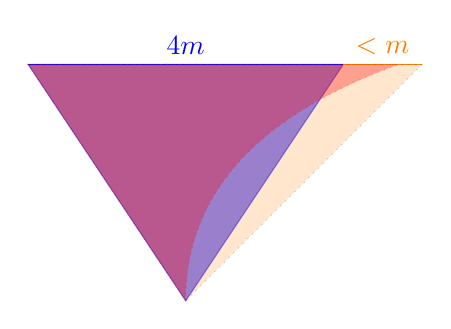
\begin{tikzpicture}
      \coordinate (r) at (0,0);
      \coordinate (b0) at (-2,3);
      \coordinate (b1) at (2,3);
      \coordinate (u) at (2.7,3);
      \coordinate (up) at (3,3);

      \draw[blue] (b0)--(b1) node[pos=0.5,above] {$4m$};
      \filldraw[draw=blue, fill=blue, opacity=0.5]
      (r)--(b0)--(b1)--cycle;
      \draw[orange] (b1)--(up) node[pos=0.5,above] {$<m$};
      \filldraw[fill=orange, opacity=0.2, dotted]
      (r)--(b0)--(up)--cycle;

      \filldraw[draw=red, fill=red, opacity=0.3, dotted] 
      (r) to[out=90, in=200] (u) -- (b0) -- cycle; 
    \end{tikzpicture}
  \end{center}
\end{frame}

\begin{frame}{Class of sets computing subsets of hyperimmune is null}
  To dominate the $k$-th element of $X$, enumerate the nodes in
  $\mathcal{U}$. Wait till a measure of $2m$ of them find $k$-elements,
  i.e. find pairwise-incomparable nodes $\tau_0,\ldots,\tau_r$ with
  $\llbracket\tau_i\rrbracket \subseteq \textcolor{red}{\mathcal{U}}$, such
  that
  \[\mu(\llbracket\tau_0\rrbracket) +\ldots
  +\mu(\llbracket\tau_k\rrbracket) \geq 2m,\]
  and
  \[\Phi^{\tau_i}_{|\tau_i|} \in 2^{<\omega}\; \text{with }
  |\Phi^{\tau_i}_{|\tau_i|}|\geq k.\]

  \vspace{2em}
  By tight approximation, such nodes exist, and one of them must be an
  initial-segment of a real that computes an infinite subset of $X$. Thus
  the $k$-th element of $X$ must be below the largest element found by all
  of these nodes. $\blacksquare$
\end{frame}

\begin{frame}{$\text{RT}_2^1$ $\nleq_{\text{soc}}$ WWKL}
  \begin{thm}
    $\text{RT}_2^1$ $\nleq_{\text{soc}}$ WWKL.
  \end{thm}

  \vspace{1em}
  \textbf{Pf:} Let $c:\omega\rightarrow\{0,1\}$ be a 2-coloring of the
  graph of a fixed bi-hyperimmune $X$, that is,
  \[c(n)=0 \Leftrightarrow n\in X.\]
  
  From hyperimmunity of $X$ and $\bar{X}$, the class of sets computing an
  infinite subset of $X$ or of $\bar{X}$ is null. Equivalently, the class
  of $c$-homogeneous sets is null. Therefore given arbitrary tree
  $T\subseteq\omega^{<\omega}$ of positive measure, some real must fail to
  compute any $c$-homogeneous set. $\blacksquare$
\end{frame}

\begin{frame}{Randomness does not imply Homogeneity}
  \begin{coro}[RT $\nleq_{\text{soc}}$ WWKL]
    $\text{RT}_2^1$ $\nleq_{\text{soc}}$ WWKL. $\blacksquare$
  \end{coro}
  \begin{coro}[WKL $\nleq_{\text{soc}}$ WWKL]
    RT $\leq_{soc}$ WKL, RT $\nleq_{\text{soc}}$ WWKL. $\blacksquare$
  \end{coro}

  \vspace{1em}
  \begin{center}
    \begin{tikzpicture}[node distance=3cm,auto,thick,>=latex']
      \node (KL) {KL$\leftrightarrow$WKL};
      \node (WWKL) [below right of=KL] {WWKL};
      \node (RT) [below left of=KL] {RT};
      \draw[->] (KL) -- (RT);
      \draw[->] (KL) -- (WWKL);
      \draw [<-,red] (RT) -- coordinate (m) (WWKL);
      \draw[shift={(m)},red](-0.1,-0.1)--(0.1,+0.1);
    \end{tikzpicture}
  \end{center}
\end{frame}
